Eget kompendium om digitale kretser.

\subsection{Kretsfamilier (Logic families)}
  Kretsfamilier refererer til forksjellige teknikker som brukes til å
implementere logikk.
\\\\
Det finnes mange av disse: RTL, DCTL, RCTL, DTL, CTDL, HTL, ECL, PECL, LVPECL,
GTL, TTL, PMOS, NMOS, HMOS, CMOS, BiCMOS, IIl.
\\\\
Heldigvis skal vi bare se på noen få av dem.



\paragraph{Bipolare komponenter (BJT)} \mbox{} \\
Dioder-vakuumrør ble brukt i de første elektroniske datamaskinene
på 1940-tallet.
\\\\
DTL, diode-transistor logikk, ble først brukt på 50-tallet når man byttet ut
vakuumrørene med transistorer.
\\\\
ECL, emitter-coupled logikk, er raske integrerte kretser som bruker for mye
energi. De ble brukt mellom 1970-1990, men kan også bli brukt i dag.
\\\\
TTL, transistor-transistor logikk, er mye brukt i integrerte kretser.
Etter oppfinnelsen på 60-tallet er de fremdeles i bruk i dag.



\paragraph{Unipolare komponenter (FET)} \mbox{} \\
FET brukes bl.a. i NMOS og CMOS kretser.
\\\\
NMOS, ulempen med NMOS er at den bruker strøm selv når den ikke switcher.
\\\\
CMOS, den mest vanlige IC-teknologien (Integrated Circuit).
Bortsett fra lekasjestrøm bruker den kun strøm når den switcher.
\\\\
BiCMOS, kombinerer CMOS og TTL.
BJT gir fordeler for analoge deler, CMOS gir enkle logiske porter.
Ble bl.a. brukt i Pentium Pro.


  \subsubsection{NMOS}
    \subsubsection{NMOS som motstand}
En NMOS kan brukes som en motstand.
Man oppnår dette ved å koble sammen Drain og Gate.
Dette kan brukes til å kontrollere logikk i diverse logiske porter.

TODO: includegraphics{nmos-resistor}

Motstanden blir da
$$R = \frac{V_{DS}}{I_D}$$
Motstanden er, som regel, i kilo-ohm og strømmen i milli-ampere.



\paragraph{NAND} \mbox \\
Man kan implementere unipolare logiske kretser med NMOS.
\\
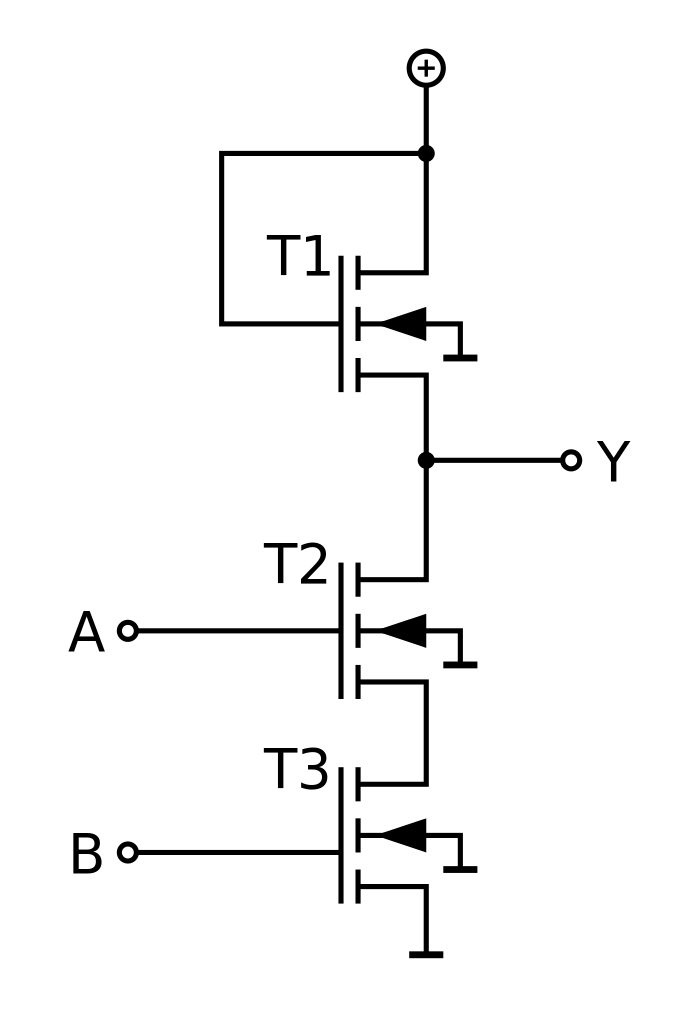
\includegraphics{./img/nmos-nand}
\\
Sannhetstabellen blir lik NAND i forige seksjon.
Når både A og B er på vil transistoren lede.
Når transistoren leder vil Y bringes ned til jord AKA null.



\paragraph{NOR} \mbox \\
NOR port implementert med NMOS.
\\
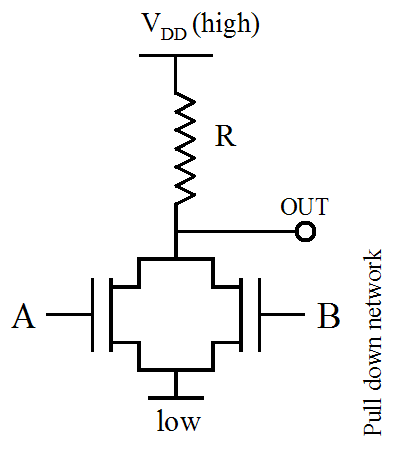
\includegraphics{./img/nmos-nor}
\\
På bildet kan man bytte ut R med en nmos-motstand (gate og drain koblet).

Hvis minst én av A eller B er på, vil transistoren lede.
Når en eller begge transistorene leder, bringes Y til jord.


  \subsubsection{DTL}
    TODO: tegn og forklar en DTL-NAND (se skrivebok)


  \subsubsection{TTL}
    TODO


\subsection{Kombinatoriske kretser}
  Vi skiller mellom kombinatoriske og sekvensielle kretser.
Noen operasjoner, som pluss og minus, er uavhengig av hva som har skjedd før.
Kombinasjonen av tall A pluss tall B gir en sum.

Ved en if-statement, if(var == 22), må man hente variable fra minne og ta en
beslutning basert på hva den variabelen var satt til.
Logikken er altså avhengig av hva som har skjedd tidligere.
Dette er sekvensiell logikk.

I denne subseksjonen skal vi se på kombinatorisk logikk hvor f.eks. summen
av to tall er uavhengig av tidligere hendelser.


  \subsubsection{Binær addisjon}
    Dette er lett å søke opp på internett.


  \subsubsection{Adders}
    TODO


\subsection{Sekvensielle kretser}
    sekvensiell TODO


  \subsubsection{Latches}
    latches n flip-flops TODO



\paragraph{SR-latch} \mbox{} \\
TODO



\paragraph{Synkron SR-latch} \mbox{} \\
TODO



\paragraph{D-latch} \mbox{} \\
TODO


  \subsubsection{Dekoder / Enkoder}
    \paragraph{Dekoder} \mbox{} \\
TODO



\paragraph{Enkoder} \mbox{} \\
TODO


  \subsubsection{ROM}
    rom TODO

